\begin{figure*}[t]
\centering
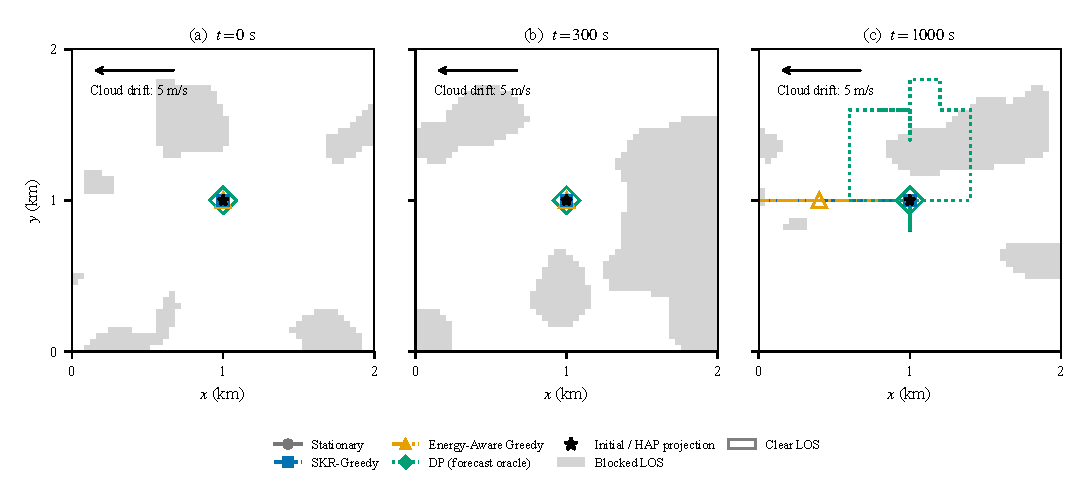
\includegraphics[width=\textwidth]{fig4_dynamic_cloud_trajectories.pdf}
\caption{UAV trajectories under dynamic cloud blockage (P2). Shading indicates sampled HAP–UAV LOS blockage for UAV coordinates on a 50-by-50 visualization grid; it is not an endpoint-cloud-cell test. Paths show saved slot endpoints up to each snapshot. Historical segments crossing a snapshot-shaded region do not imply blockage at their traversal times; continuous inter-slot LOS clearance is not certified. Cloud drift is (-5, 0) m/s. All methods share the initial point and HAP ground projection. Coincident current positions use nested markers. DP uses a perfect future-cloud forecast; greedy actions are myopic. Phase 6A numerical diagnostic, not security-certified results.}
\label{fig:phase6a-4}
\end{figure*}

\begin{figure}[t]
\centering
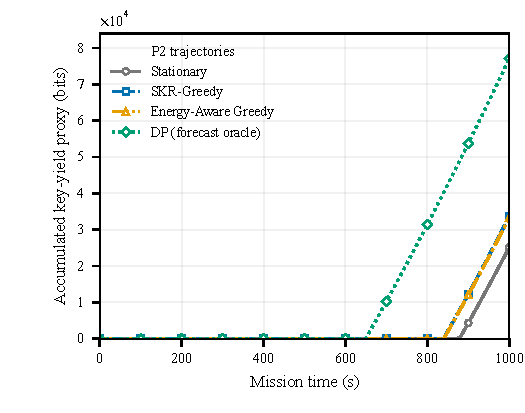
\includegraphics[width=\columnwidth]{fig5_accumulated_key_vs_time.pdf}
\caption{Accumulated finite-size key-yield proxy versus mission time along saved P2 trajectories. A single finite-size correction is applied to each accumulated prefix; curves are not linear ramps from terminal average rates. Phase 6A uses 100 slots of 10 s. P1 selects the same saved paths in this scenario. DP is a forecast oracle; the proxy is not a composable-security proof.}
\label{fig:phase6a-5}
\end{figure}

\begin{figure}[t]
\centering
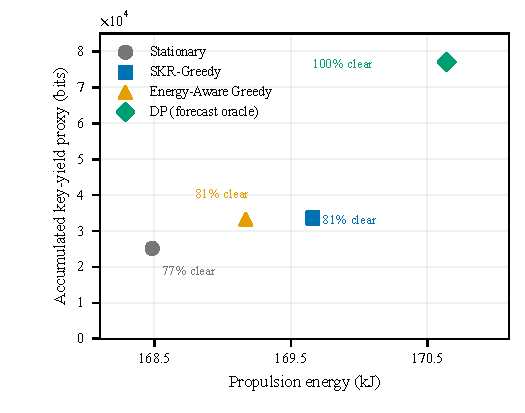
\includegraphics[width=\columnwidth]{fig7_energy_key_tradeoff.pdf}
\caption{Propulsion energy versus accumulated finite-size key-yield proxy for the four saved P2 trajectories at one nonbinding budget. Percentages indicate sampled clear-LOS fractions. Points are not connected and do not define a Pareto frontier. DP produces more key while consuming more energy and has perfect future-cloud information.}
\label{fig:phase6a-7}
\end{figure}

% Fig.6 pending matched-budget experiments; no placeholder graphic.